\section{Zustandsraumdarstellung (ZRD)}

\textbf{Grundidee:} Differentialgleichung $n.$ Ordnung eines Systems durch ein \textbf{Differentialgleichungssystem} 
von $n$ Gleichungen $1.$ Ordnung darzustellen.


\subsection{Vorteile der ZRD}{253-254}
\begin{itemize}
    \item Innere Systemstabilitäten können erkannt werden, di ebie der Untersuchung der UTF 
        nicht festgestellt werden können \textrightarrow\ Einblick in den \textbf{inneren Aufbau} eines Systems
    \item Wichtig in der Regelungstechnik
    \item ZRD hat Vorteile bei der \textbf{numerischen} Behandlung von Systemen
    \item Beschreibung durch \textbf{Energiespeicher}, in der Elektrotechnik L und C
    \item \textbf{Nur Integratoren} werden verwendet, keine Differentiatoren
\end{itemize}


\subsection{Zustandsraumdarstellung (ZRD) im Zeitbereich}{255}

\begin{minipage}[c]{0.4\columnwidth}
    \vspace{-0.3cm}
    
    \begin{empheq}[box=\fbox] {align*}
        \underline{\dot{x}}(t) &= \bm{A} \underline{x}(t) + \bm{B} \underline{u}(t) \\
        \underline{y}(t) &= \bm{C} \underline{x}(t) + \bm{D} \underline{u}(t)
    \end{empheq}

    \begin{tabular}{ll@{}}
        $\underline{u}(t)$   & Eingangsvektor ($m$ Zeilen) \\
        $\underline{x}(t)$   & Zustandsvektor ($n$ Zeilen) \\
        $\underline{y}(t)$   & Ausgangsvektor ($k$ Zeilen) \\
    \end{tabular}

\end{minipage}
\hfill
\begin{minipage}[c]{0.58\columnwidth}
    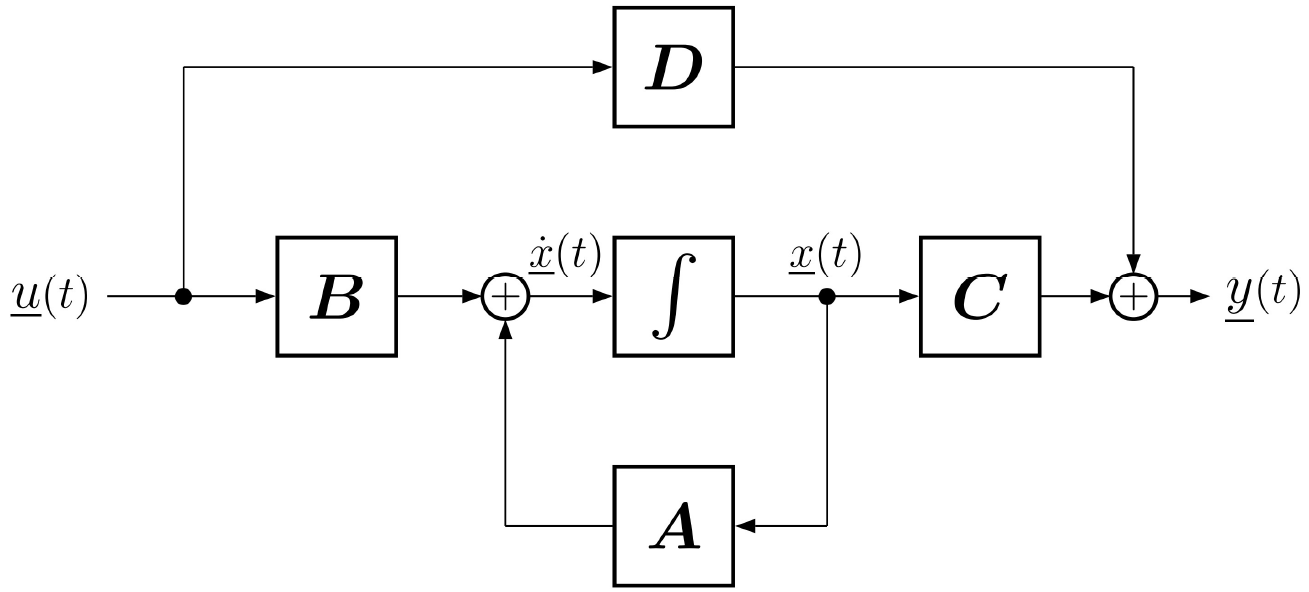
\includegraphics[width=\columnwidth]{images/blockdiagramm_zustandsdarstellung.png}
\end{minipage}


\begin{itemize}
    \item obere Gleichung: \textbf{Zustandsgleichung}
    \item untere Gleichung: \textbf{Ausgangsgleichung}
    \item $\bm{A}$ \textbf{Systemmatrix} ($n \times n$-Matrix) \\
        Sie bestimmt das Verhalten des \textbf{ungestörten Systems} ($\underline{u}(t) = 0$)
        und bestimmt z.B. die innere Stabilität des gesamten Systems.
    \item $\bm{B}$ \textbf{Eingangsmatrix (Steuermatrix)} ($n \times m$-Matrix) \\
        Sie bestimmt die Wirkung der \textbf{Steuergrössen} $\underline{u}(t)$ auf die \textbf{Zustandsgrössen} $\underline{x}(t)$
    \item $\bm{C}$ \textbf{Ausgangsmatrix (Beobachtungsmatrix)} ($k \times n$-Matrix) \\
        Sie kennzeichnet die Anhängigkeit des \textbf{Zustandes} $\underline{x}(t)$ vonder beobachtbaren Ausgangsgrösse $\underline{y}(t)$
    \item $\bm{D}$ \textbf{Durchgangsmatrix} ($k \times m$-Matrix) \\
        Sie bestimmt die unmittelbare Wirkung der Eingangsgrösse $\underline{u}(t)$ auf den Ausgang $\underline{y}(t)$
\end{itemize}


\subsection{Ordnung eines Systems}{256}

Die \textbf{Ordnung} eines Systems definiert die\textbf{kleinste Anzahl von Zustandsgrössen} $x(t)$.
Äquivalent dazu kann die Ordnung eines Systems auch als die \textbf{Anzahl der unabhängigen Energiespeicher} definiert werden.


\subsection{Zustandsraumdarstellung (ZRD) im Laplace-Bereich}{264}

\begin{minipage}[c]{0.44\columnwidth}
    \vspace{-0.3cm}
    
    \begin{empheq}[box=\fbox] {align*}
        s \underline{X}(s) - x(0) &= \bm{A} \underline{X}(s) + \bm{B} \underline{U}(s) \\
        \underline{Y}(s) &= \bm{C} \underline{X}(s) + \bm{D} \underline{U}(s)
    \end{empheq}

    \begin{tabular}{ll@{}}
        $\underline{U}(s)$   & Eingangsvektor ($m$ Zeilen) \\
        $\underline{X}(s)$   & Zustandsvektor ($n$ Zeilen) \\
        $\underline{Y}(s)$   & Ausgangsvektor ($k$ Zeilen) \\
        $\bm{I}$             & Einheitsmatrix \\
        $\bm{H(s)}$          & Übertragungsmatrix \\
    \end{tabular}

\end{minipage}
\hfill
\begin{minipage}[c]{0.54\columnwidth}
    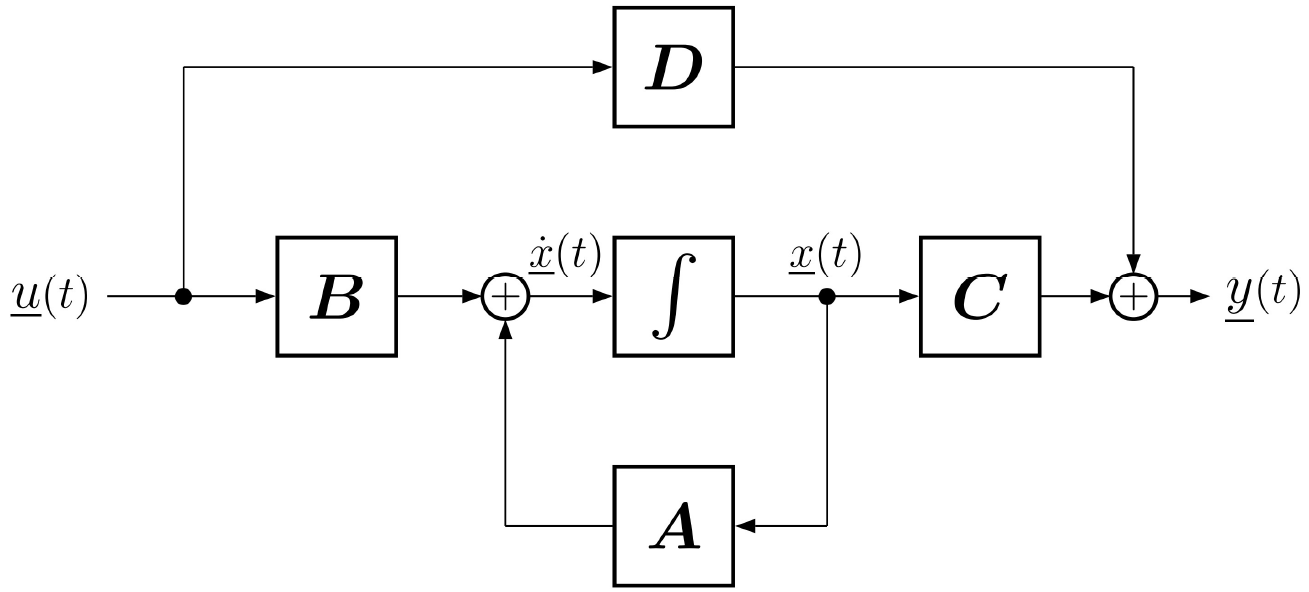
\includegraphics[width=\columnwidth]{images/blockdiagramm_zustandsdarstellung.png}
\end{minipage}

\vspace{0.2cm}
$$ \boxed{ \underline{Y}(s) = \bm{C}(s \bm{I} - \bm{A})^{-1} \underline{x}(0) 
    + \underbrace{(\bm{C}(s \bm{I} - \bm{A})^{-1} \bm{B} + \bm{D} )}_{\bm{H(s)}} \underline{U}(s) } $$

Mit Anfangsbedingungen $x(0) = 0$ ergibt sich folgender Zusammenhang, was der Übertragungsfunktion (UTF) entspricht,
aber im allgemeinen Fall eine \textbf{Matrix} ist.
$$ \boxed{ \underline{Y}(s) = \underbrace{(\bm{C}(s \bm{I} - \bm{A})^{-1} \bm{B} + \bm{D} )}_{\bm{H(s)}} \underline{U}(s) } $$

\textbf{Hinweis:} Aus einem Signalflussdiagramm (SFD) ist es meist sehr einfach, die gesuchten Grössen der ZRD zu finden.


\subsubsection{Übertragungsmatrix und Übertragungsfunktion}{266}

\begin{minipage}[t]{0.48\columnwidth}
    \begin{center}
        \textbf{\myul{Übertragungsmatrix}}
    \end{center}
    \begin{itemize}
        \item MIMO-Systeme
        \item Beschreibung in Matritzenform
            $$ Y(s) = \bm{H(s)} \cdot U(s) $$
        \item  $H(s)$ hat gleiche Grösse (Dimensionen) wie Durchgangsmatrix $\bm{D}$
    \end{itemize}
\end{minipage}
\hfill
\begin{minipage}[t]{0.48\columnwidth}
    \begin{center}
        \textbf{\myul{Übertragungsfunktion}}
    \end{center}
        \begin{itemize}
            \item SISO-Systeme
            \item Matrix-Form wird zu 'normaler' Gleichung
            $$ Y(s) = H(s) \cdot U(s) $$
        \end{itemize}
\end{minipage}